
%(BEGIN_QUESTION)
% Copyright 2012, Tony R. Kuphaldt, released under the Creative Commons Attribution License (v 1.0)
% This means you may do almost anything with this work of mine, so long as you give me proper credit

Many flammable gases are produced in chemical processing and oil refineries as ``waste'' products.  These ``waste'' gases may be used as fuel for steam boilers and combustion heaters in other parts of the refinery.  The problem is, ``waste'' fuel gas production is often unsteady, and the demand for fuel gas in boilers and heaters is unsteady as well.  There are times when there will be a surplus of waste gas (more than can be used), and times when there will not be enough.

The following pressure control system works to maintain constant fuel gas pressure in the accumulator vessel despite changes in waste gas flows and fuel gas demands:

$$\includegraphics[width=15.5cm]{i01263x01.eps}$$

A pair of split-ranged control valves (PV-45a and PV-45b) work together to either admit natural gas into the accumulator (when the gas pressure is too low) or release excess gas to the flare (when pressure is too high).

\vskip 10pt

Operations personnel have determined that the pressure inside this accumulator is not steady enough for their operational needs.  They have also determined that fast-changing waste gas flows are the source of the instability, and so they ask instrumentation personnel to implement a solution.  The instrumentation personnel, in turn, decide to implement a {\it feedforward} control strategy to meet this need.

The first step, of course, is to install flowmeters on each of the waste gas lines entering the accumulator, the signals of which will be used in the feedforward strategy to proactively compensate for changes in waste gas flows.  A controversy erupts between instrumentation personnel, however, regarding how to implement the feedfoward strategy.

\filbreak

One team says the strategy should look like this:

$$\includegraphics[width=15.5cm]{i01263x02.eps}$$

Another team says the strategy should look like this:

$$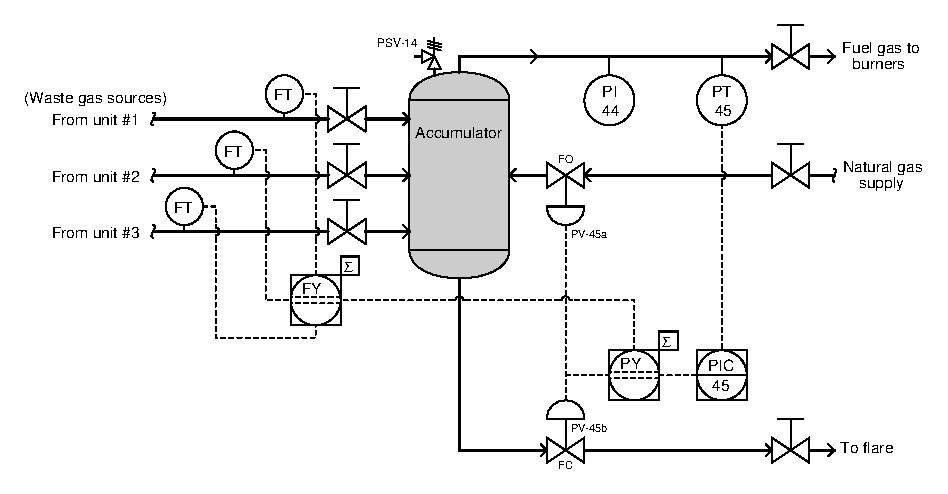
\includegraphics[width=15.5cm]{i01263x03.eps}$$

Which team do you agree with, and why?  Note: {\it this is a very important concept to grasp in feedforward control strategies, and in fact is one of the most commonly mis-understood concepts associated with feedforward!}

\vskip 10pt

\underbar{file i01263}
%(END_QUESTION)





%(BEGIN_ANSWER)

This is the correct solution, where the total load flow signal gets added to the {\it output} of the pressure controller, not to its {\it PV input}:
 
$$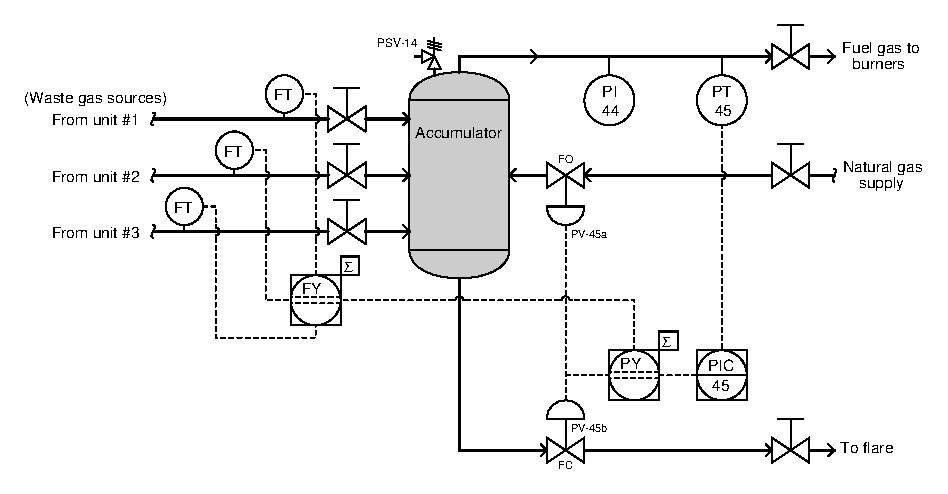
\includegraphics[width=15.5cm]{i01263x03.eps}$$

The reason for this is quite straightforward: we want the feedforward signal to directly contribute to the positions of the control valves, so that any change in waste gas flow immediately biases the control valves in order to proactively compensate.  If the feedforward signal were to be added to the pressure controller's PV signal, it would cause the pressure controller to incorrectly see changes in pressure that were really changes in waste gas flow.  Not only would this not achieve the desired effect, but it would also ``lie'' to the pressure controller, the result of which being it could never properly hold to setpoint!

%(END_ANSWER)





%(BEGIN_NOTES)

$$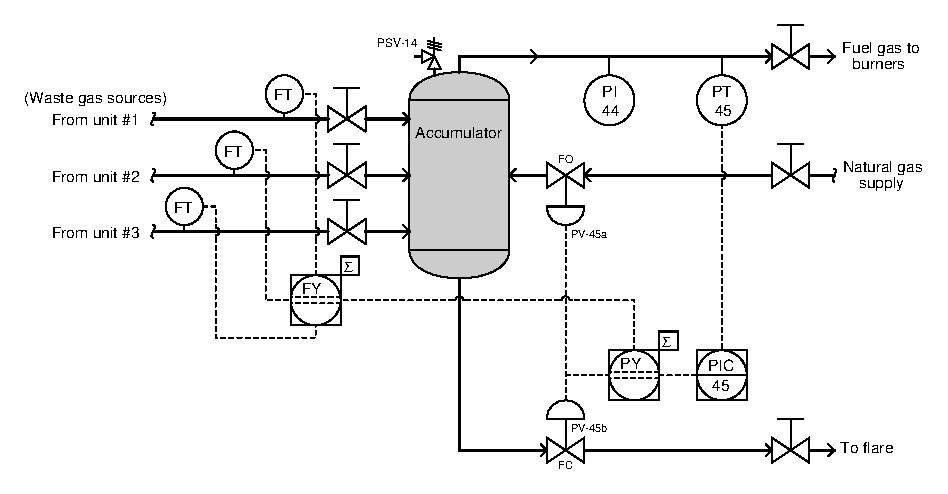
\includegraphics[width=15.5cm]{i01263x03.eps}$$

\vskip 20pt \vbox{\hrule \hbox{\strut \vrule{} {\bf Virtual Troubleshooting} \vrule} \hrule}

\noindent
{\bf Predicting the effect of a given fault:} present each of the following faults to the students, one at a time, having them comment on all the effects each fault would produce.

\begin{itemize}
\item{} 
\item{} 
\item{} 
\end{itemize}


\vskip 10pt


\noindent
{\bf Identifying possible/impossible faults:} present symptoms to the students and then have them determine whether or not a series of suggested faults could account for all the symptoms, explaining {\it why} or {\it why not} for each proposed fault:

\begin{itemize}
\item{} Symptom: {\it }
\item{}  -- {\bf Yes/No}
\item{}  -- {\bf Yes/No}
\item{}  -- {\bf Yes/No}
\end{itemize}


\vskip 10pt

\filbreak


\noindent
{\bf Determining the utility of given diagnostic tests:} present symptoms to the students and then propose the following diagnostic tests one by one.  Students rate the value of each test, determining whether or not it would give useful information (i.e. tell us something we don't already know).  Students determine what different results for each test would indicate about the fault, if anything:

\begin{itemize}
\item{} Symptom: {\it PT-45 shows an oscillating pressure}
\item{} Check gain values in FY summer -- {\bf No}
\item{} Check gain value of PIC-45 summer -- {\bf Yes}
\item{} Check PI-44 indication to see if it's oscillating too -- {\bf No} (highly unlikely that PT-45 is oscillating on its own)
\item{} Examine phase shift between PV and Output of PIC-45 -- {\bf Yes}
\item{} Plot load flows on a trend graph -- {\bf Yes}
\end{itemize}


\vskip 10pt


\noindent
{\bf Diagnosing a fault based on given symptoms:} imagine the ??? fails ??? in this system (don't reveal the fault to students!).  Present the operator's observation(s) to the students, have them consider possible faults and diagnostic strategies, and then tell them the results of tests they propose based on the following symptoms, until they have properly identified the nature and location of the fault:

\begin{itemize}
\item{} Operator observation: {\it }
\item{} 
\item{} 
\end{itemize}
%INDEX% Control, strategies: feedforward (gas accumulator pressure control)

%(END_NOTES)


